% AUTO-GENERATED by writeup/make_rehaul_factor.py -- do not edit; re-run the script.
\ifdefined\rhfaReading\else% AUTO-GENERATED by writeup/make_rehaul_factor.py -- do not edit; re-run the script.
% \rhfa... macros: factor-augmented HAR (diffusion index) on Table 1's design (results/channels_2026-10-26/
% RULE.txt section 4; results/channels_2026-10-26/factor).  Spans: Ord = ORDINARY days (primary), All = every
% bar, Ev = the 81 FOMC statement days.  Models: Pca<k>, Pls<k>, Full (the span's L_full model).
\providecommand{\rhfaPcaOneOrdPct}{}\renewcommand{\rhfaPcaOneOrdPct}{0.08}  % pca1 ordinary: QLIKE change vs OLS-HAR, %
\providecommand{\rhfaPcaOneOrdMsePct}{}\renewcommand{\rhfaPcaOneOrdMsePct}{3.28}  % pca1 ordinary: MSE change vs OLS-HAR, %
\providecommand{\rhfaPcaOneOrdDm}{}\renewcommand{\rhfaPcaOneOrdDm}{0.90}  % pca1 ordinary: DM vs OLS-HAR (QLIKE)
\providecommand{\rhfaPcaOneOrdP}{}\renewcommand{\rhfaPcaOneOrdP}{0.369}  % pca1 ordinary: p
\providecommand{\rhfaPcaOneOrdDmFull}{}\renewcommand{\rhfaPcaOneOrdDmFull}{4.89}  % pca1 ordinary: DM vs the full set (enet)
\providecommand{\rhfaPcaOneOrdPFull}{}\renewcommand{\rhfaPcaOneOrdPFull}{$<$0.001}  % pca1 ordinary: p
\providecommand{\rhfaPcaOneOrdR}{}\renewcommand{\rhfaPcaOneOrdR}{$-$0.02}  % pca1 ordinary: R_k
\providecommand{\rhfaPcaTwoOrdPct}{}\renewcommand{\rhfaPcaTwoOrdPct}{0.06}  % pca2 ordinary: QLIKE change vs OLS-HAR, %
\providecommand{\rhfaPcaTwoOrdMsePct}{}\renewcommand{\rhfaPcaTwoOrdMsePct}{1.85}  % pca2 ordinary: MSE change vs OLS-HAR, %
\providecommand{\rhfaPcaTwoOrdDm}{}\renewcommand{\rhfaPcaTwoOrdDm}{0.32}  % pca2 ordinary: DM vs OLS-HAR (QLIKE)
\providecommand{\rhfaPcaTwoOrdP}{}\renewcommand{\rhfaPcaTwoOrdP}{0.748}  % pca2 ordinary: p
\providecommand{\rhfaPcaTwoOrdDmFull}{}\renewcommand{\rhfaPcaTwoOrdDmFull}{4.86}  % pca2 ordinary: DM vs the full set (enet)
\providecommand{\rhfaPcaTwoOrdPFull}{}\renewcommand{\rhfaPcaTwoOrdPFull}{$<$0.001}  % pca2 ordinary: p
\providecommand{\rhfaPcaTwoOrdR}{}\renewcommand{\rhfaPcaTwoOrdR}{$-$0.02}  % pca2 ordinary: R_k
\providecommand{\rhfaPcaThreeOrdPct}{}\renewcommand{\rhfaPcaThreeOrdPct}{0.45}  % pca3 ordinary: QLIKE change vs OLS-HAR, %
\providecommand{\rhfaPcaThreeOrdMsePct}{}\renewcommand{\rhfaPcaThreeOrdMsePct}{5.76}  % pca3 ordinary: MSE change vs OLS-HAR, %
\providecommand{\rhfaPcaThreeOrdDm}{}\renewcommand{\rhfaPcaThreeOrdDm}{1.44}  % pca3 ordinary: DM vs OLS-HAR (QLIKE)
\providecommand{\rhfaPcaThreeOrdP}{}\renewcommand{\rhfaPcaThreeOrdP}{0.151}  % pca3 ordinary: p
\providecommand{\rhfaPcaThreeOrdDmFull}{}\renewcommand{\rhfaPcaThreeOrdDmFull}{5.33}  % pca3 ordinary: DM vs the full set (enet)
\providecommand{\rhfaPcaThreeOrdPFull}{}\renewcommand{\rhfaPcaThreeOrdPFull}{$<$0.001}  % pca3 ordinary: p
\providecommand{\rhfaPcaThreeOrdR}{}\renewcommand{\rhfaPcaThreeOrdR}{$-$0.11}  % pca3 ordinary: R_k
\providecommand{\rhfaPcaFiveOrdPct}{}\renewcommand{\rhfaPcaFiveOrdPct}{0.93}  % pca5 ordinary: QLIKE change vs OLS-HAR, %
\providecommand{\rhfaPcaFiveOrdMsePct}{}\renewcommand{\rhfaPcaFiveOrdMsePct}{3.77}  % pca5 ordinary: MSE change vs OLS-HAR, %
\providecommand{\rhfaPcaFiveOrdDm}{}\renewcommand{\rhfaPcaFiveOrdDm}{1.85}  % pca5 ordinary: DM vs OLS-HAR (QLIKE)
\providecommand{\rhfaPcaFiveOrdP}{}\renewcommand{\rhfaPcaFiveOrdP}{0.064}  % pca5 ordinary: p
\providecommand{\rhfaPcaFiveOrdDmFull}{}\renewcommand{\rhfaPcaFiveOrdDmFull}{5.94}  % pca5 ordinary: DM vs the full set (enet)
\providecommand{\rhfaPcaFiveOrdPFull}{}\renewcommand{\rhfaPcaFiveOrdPFull}{$<$0.001}  % pca5 ordinary: p
\providecommand{\rhfaPcaFiveOrdR}{}\renewcommand{\rhfaPcaFiveOrdR}{$-$0.23}  % pca5 ordinary: R_k
\providecommand{\rhfaPcaTenOrdPct}{}\renewcommand{\rhfaPcaTenOrdPct}{$-$1.06}  % pca10 ordinary: QLIKE change vs OLS-HAR, %
\providecommand{\rhfaPcaTenOrdMsePct}{}\renewcommand{\rhfaPcaTenOrdMsePct}{21.39}  % pca10 ordinary: MSE change vs OLS-HAR, %
\providecommand{\rhfaPcaTenOrdDm}{}\renewcommand{\rhfaPcaTenOrdDm}{$-$2.19}  % pca10 ordinary: DM vs OLS-HAR (QLIKE)
\providecommand{\rhfaPcaTenOrdP}{}\renewcommand{\rhfaPcaTenOrdP}{0.028}  % pca10 ordinary: p
\providecommand{\rhfaPcaTenOrdDmFull}{}\renewcommand{\rhfaPcaTenOrdDmFull}{4.45}  % pca10 ordinary: DM vs the full set (enet)
\providecommand{\rhfaPcaTenOrdPFull}{}\renewcommand{\rhfaPcaTenOrdPFull}{$<$0.001}  % pca10 ordinary: p
\providecommand{\rhfaPcaTenOrdR}{}\renewcommand{\rhfaPcaTenOrdR}{0.27}  % pca10 ordinary: R_k
\providecommand{\rhfaPcaTwentyOrdPct}{}\renewcommand{\rhfaPcaTwentyOrdPct}{$-$1.09}  % pca20 ordinary: QLIKE change vs OLS-HAR, %
\providecommand{\rhfaPcaTwentyOrdMsePct}{}\renewcommand{\rhfaPcaTwentyOrdMsePct}{45.47}  % pca20 ordinary: MSE change vs OLS-HAR, %
\providecommand{\rhfaPcaTwentyOrdDm}{}\renewcommand{\rhfaPcaTwentyOrdDm}{$-$1.53}  % pca20 ordinary: DM vs OLS-HAR (QLIKE)
\providecommand{\rhfaPcaTwentyOrdP}{}\renewcommand{\rhfaPcaTwentyOrdP}{0.126}  % pca20 ordinary: p
\providecommand{\rhfaPcaTwentyOrdDmFull}{}\renewcommand{\rhfaPcaTwentyOrdDmFull}{3.66}  % pca20 ordinary: DM vs the full set (enet)
\providecommand{\rhfaPcaTwentyOrdPFull}{}\renewcommand{\rhfaPcaTwentyOrdPFull}{$<$0.001}  % pca20 ordinary: p
\providecommand{\rhfaPcaTwentyOrdR}{}\renewcommand{\rhfaPcaTwentyOrdR}{0.27}  % pca20 ordinary: R_k
\providecommand{\rhfaPlsOneOrdPct}{}\renewcommand{\rhfaPlsOneOrdPct}{0.01}  % pls1 ordinary: QLIKE change vs OLS-HAR, %
\providecommand{\rhfaPlsOneOrdMsePct}{}\renewcommand{\rhfaPlsOneOrdMsePct}{14.31}  % pls1 ordinary: MSE change vs OLS-HAR, %
\providecommand{\rhfaPlsOneOrdDm}{}\renewcommand{\rhfaPlsOneOrdDm}{0.05}  % pls1 ordinary: DM vs OLS-HAR (QLIKE)
\providecommand{\rhfaPlsOneOrdP}{}\renewcommand{\rhfaPlsOneOrdP}{0.962}  % pls1 ordinary: p
\providecommand{\rhfaPlsOneOrdDmFull}{}\renewcommand{\rhfaPlsOneOrdDmFull}{4.95}  % pls1 ordinary: DM vs the full set (enet)
\providecommand{\rhfaPlsOneOrdPFull}{}\renewcommand{\rhfaPlsOneOrdPFull}{$<$0.001}  % pls1 ordinary: p
\providecommand{\rhfaPlsOneOrdR}{}\renewcommand{\rhfaPlsOneOrdR}{0.00}  % pls1 ordinary: R_k
\providecommand{\rhfaPlsTwoOrdPct}{}\renewcommand{\rhfaPlsTwoOrdPct}{1.57}  % pls2 ordinary: QLIKE change vs OLS-HAR, %
\providecommand{\rhfaPlsTwoOrdMsePct}{}\renewcommand{\rhfaPlsTwoOrdMsePct}{24.30}  % pls2 ordinary: MSE change vs OLS-HAR, %
\providecommand{\rhfaPlsTwoOrdDm}{}\renewcommand{\rhfaPlsTwoOrdDm}{1.29}  % pls2 ordinary: DM vs OLS-HAR (QLIKE)
\providecommand{\rhfaPlsTwoOrdP}{}\renewcommand{\rhfaPlsTwoOrdP}{0.196}  % pls2 ordinary: p
\providecommand{\rhfaPlsTwoOrdDmFull}{}\renewcommand{\rhfaPlsTwoOrdDmFull}{4.51}  % pls2 ordinary: DM vs the full set (enet)
\providecommand{\rhfaPlsTwoOrdPFull}{}\renewcommand{\rhfaPlsTwoOrdPFull}{$<$0.001}  % pls2 ordinary: p
\providecommand{\rhfaPlsTwoOrdR}{}\renewcommand{\rhfaPlsTwoOrdR}{$-$0.40}  % pls2 ordinary: R_k
\providecommand{\rhfaPlsThreeOrdPct}{}\renewcommand{\rhfaPlsThreeOrdPct}{0.04}  % pls3 ordinary: QLIKE change vs OLS-HAR, %
\providecommand{\rhfaPlsThreeOrdMsePct}{}\renewcommand{\rhfaPlsThreeOrdMsePct}{99.04}  % pls3 ordinary: MSE change vs OLS-HAR, %
\providecommand{\rhfaPlsThreeOrdDm}{}\renewcommand{\rhfaPlsThreeOrdDm}{0.03}  % pls3 ordinary: DM vs OLS-HAR (QLIKE)
\providecommand{\rhfaPlsThreeOrdP}{}\renewcommand{\rhfaPlsThreeOrdP}{0.974}  % pls3 ordinary: p
\providecommand{\rhfaPlsThreeOrdDmFull}{}\renewcommand{\rhfaPlsThreeOrdDmFull}{3.84}  % pls3 ordinary: DM vs the full set (enet)
\providecommand{\rhfaPlsThreeOrdPFull}{}\renewcommand{\rhfaPlsThreeOrdPFull}{$<$0.001}  % pls3 ordinary: p
\providecommand{\rhfaPlsThreeOrdR}{}\renewcommand{\rhfaPlsThreeOrdR}{$-$0.01}  % pls3 ordinary: R_k
\providecommand{\rhfaFullOrdModel}{}\renewcommand{\rhfaFullOrdModel}{elastic net}  % ordinary: L_full model (lower QLIKE of ridge, elastic net)
\providecommand{\rhfaFullOrdPct}{}\renewcommand{\rhfaFullOrdPct}{$-$3.97}  % ordinary: full set QLIKE change vs OLS-HAR, %
\providecommand{\rhfaFullOrdMsePct}{}\renewcommand{\rhfaFullOrdMsePct}{128.86}  % ordinary: full set MSE change vs OLS-HAR, %
\providecommand{\rhfaFullOrdDm}{}\renewcommand{\rhfaFullOrdDm}{$-$4.73}  % ordinary: full set DM vs OLS-HAR
\providecommand{\rhfaFullOrdP}{}\renewcommand{\rhfaFullOrdP}{$<$0.001}  % ordinary: p
\providecommand{\rhfaNOrdDays}{}\renewcommand{\rhfaNOrdDays}{2{,}498}  % ordinary: days
\providecommand{\rhfaNOrdBars}{}\renewcommand{\rhfaNOrdBars}{32{,}474}  % ordinary: bars
\providecommand{\rhfaPcaOneAllPct}{}\renewcommand{\rhfaPcaOneAllPct}{$-$0.05}  % pca1 all: QLIKE change vs OLS-HAR, %
\providecommand{\rhfaPcaOneAllMsePct}{}\renewcommand{\rhfaPcaOneAllMsePct}{3.00}  % pca1 all: MSE change vs OLS-HAR, %
\providecommand{\rhfaPcaOneAllDm}{}\renewcommand{\rhfaPcaOneAllDm}{$-$0.53}  % pca1 all: DM vs OLS-HAR (QLIKE)
\providecommand{\rhfaPcaOneAllP}{}\renewcommand{\rhfaPcaOneAllP}{0.595}  % pca1 all: p
\providecommand{\rhfaPcaOneAllDmFull}{}\renewcommand{\rhfaPcaOneAllDmFull}{7.44}  % pca1 all: DM vs the full set (enet)
\providecommand{\rhfaPcaOneAllPFull}{}\renewcommand{\rhfaPcaOneAllPFull}{$<$0.001}  % pca1 all: p
\providecommand{\rhfaPcaOneAllR}{}\renewcommand{\rhfaPcaOneAllR}{0.01}  % pca1 all: R_k
\providecommand{\rhfaPcaTwoAllPct}{}\renewcommand{\rhfaPcaTwoAllPct}{0.11}  % pca2 all: QLIKE change vs OLS-HAR, %
\providecommand{\rhfaPcaTwoAllMsePct}{}\renewcommand{\rhfaPcaTwoAllMsePct}{1.71}  % pca2 all: MSE change vs OLS-HAR, %
\providecommand{\rhfaPcaTwoAllDm}{}\renewcommand{\rhfaPcaTwoAllDm}{0.55}  % pca2 all: DM vs OLS-HAR (QLIKE)
\providecommand{\rhfaPcaTwoAllP}{}\renewcommand{\rhfaPcaTwoAllP}{0.579}  % pca2 all: p
\providecommand{\rhfaPcaTwoAllDmFull}{}\renewcommand{\rhfaPcaTwoAllDmFull}{7.48}  % pca2 all: DM vs the full set (enet)
\providecommand{\rhfaPcaTwoAllPFull}{}\renewcommand{\rhfaPcaTwoAllPFull}{$<$0.001}  % pca2 all: p
\providecommand{\rhfaPcaTwoAllR}{}\renewcommand{\rhfaPcaTwoAllR}{$-$0.02}  % pca2 all: R_k
\providecommand{\rhfaPcaThreeAllPct}{}\renewcommand{\rhfaPcaThreeAllPct}{0.69}  % pca3 all: QLIKE change vs OLS-HAR, %
\providecommand{\rhfaPcaThreeAllMsePct}{}\renewcommand{\rhfaPcaThreeAllMsePct}{5.30}  % pca3 all: MSE change vs OLS-HAR, %
\providecommand{\rhfaPcaThreeAllDm}{}\renewcommand{\rhfaPcaThreeAllDm}{2.24}  % pca3 all: DM vs OLS-HAR (QLIKE)
\providecommand{\rhfaPcaThreeAllP}{}\renewcommand{\rhfaPcaThreeAllP}{0.025}  % pca3 all: p
\providecommand{\rhfaPcaThreeAllDmFull}{}\renewcommand{\rhfaPcaThreeAllDmFull}{7.96}  % pca3 all: DM vs the full set (enet)
\providecommand{\rhfaPcaThreeAllPFull}{}\renewcommand{\rhfaPcaThreeAllPFull}{$<$0.001}  % pca3 all: p
\providecommand{\rhfaPcaThreeAllR}{}\renewcommand{\rhfaPcaThreeAllR}{$-$0.10}  % pca3 all: R_k
\providecommand{\rhfaPcaFiveAllPct}{}\renewcommand{\rhfaPcaFiveAllPct}{0.94}  % pca5 all: QLIKE change vs OLS-HAR, %
\providecommand{\rhfaPcaFiveAllMsePct}{}\renewcommand{\rhfaPcaFiveAllMsePct}{3.39}  % pca5 all: MSE change vs OLS-HAR, %
\providecommand{\rhfaPcaFiveAllDm}{}\renewcommand{\rhfaPcaFiveAllDm}{2.05}  % pca5 all: DM vs OLS-HAR (QLIKE)
\providecommand{\rhfaPcaFiveAllP}{}\renewcommand{\rhfaPcaFiveAllP}{0.041}  % pca5 all: p
\providecommand{\rhfaPcaFiveAllDmFull}{}\renewcommand{\rhfaPcaFiveAllDmFull}{8.48}  % pca5 all: DM vs the full set (enet)
\providecommand{\rhfaPcaFiveAllPFull}{}\renewcommand{\rhfaPcaFiveAllPFull}{$<$0.001}  % pca5 all: p
\providecommand{\rhfaPcaFiveAllR}{}\renewcommand{\rhfaPcaFiveAllR}{$-$0.14}  % pca5 all: R_k
\providecommand{\rhfaPcaTenAllPct}{}\renewcommand{\rhfaPcaTenAllPct}{$-$0.66}  % pca10 all: QLIKE change vs OLS-HAR, %
\providecommand{\rhfaPcaTenAllMsePct}{}\renewcommand{\rhfaPcaTenAllMsePct}{19.64}  % pca10 all: MSE change vs OLS-HAR, %
\providecommand{\rhfaPcaTenAllDm}{}\renewcommand{\rhfaPcaTenAllDm}{$-$1.43}  % pca10 all: DM vs OLS-HAR (QLIKE)
\providecommand{\rhfaPcaTenAllP}{}\renewcommand{\rhfaPcaTenAllP}{0.152}  % pca10 all: p
\providecommand{\rhfaPcaTenAllDmFull}{}\renewcommand{\rhfaPcaTenAllDmFull}{7.31}  % pca10 all: DM vs the full set (enet)
\providecommand{\rhfaPcaTenAllPFull}{}\renewcommand{\rhfaPcaTenAllPFull}{$<$0.001}  % pca10 all: p
\providecommand{\rhfaPcaTenAllR}{}\renewcommand{\rhfaPcaTenAllR}{0.10}  % pca10 all: R_k
\providecommand{\rhfaPcaTwentyAllPct}{}\renewcommand{\rhfaPcaTwentyAllPct}{$-$0.87}  % pca20 all: QLIKE change vs OLS-HAR, %
\providecommand{\rhfaPcaTwentyAllMsePct}{}\renewcommand{\rhfaPcaTwentyAllMsePct}{41.73}  % pca20 all: MSE change vs OLS-HAR, %
\providecommand{\rhfaPcaTwentyAllDm}{}\renewcommand{\rhfaPcaTwentyAllDm}{$-$1.28}  % pca20 all: DM vs OLS-HAR (QLIKE)
\providecommand{\rhfaPcaTwentyAllP}{}\renewcommand{\rhfaPcaTwentyAllP}{0.201}  % pca20 all: p
\providecommand{\rhfaPcaTwentyAllDmFull}{}\renewcommand{\rhfaPcaTwentyAllDmFull}{6.40}  % pca20 all: DM vs the full set (enet)
\providecommand{\rhfaPcaTwentyAllPFull}{}\renewcommand{\rhfaPcaTwentyAllPFull}{$<$0.001}  % pca20 all: p
\providecommand{\rhfaPcaTwentyAllR}{}\renewcommand{\rhfaPcaTwentyAllR}{0.13}  % pca20 all: R_k
\providecommand{\rhfaPlsOneAllPct}{}\renewcommand{\rhfaPlsOneAllPct}{$-$0.23}  % pls1 all: QLIKE change vs OLS-HAR, %
\providecommand{\rhfaPlsOneAllMsePct}{}\renewcommand{\rhfaPlsOneAllMsePct}{13.12}  % pls1 all: MSE change vs OLS-HAR, %
\providecommand{\rhfaPlsOneAllDm}{}\renewcommand{\rhfaPlsOneAllDm}{$-$1.07}  % pls1 all: DM vs OLS-HAR (QLIKE)
\providecommand{\rhfaPlsOneAllP}{}\renewcommand{\rhfaPlsOneAllP}{0.284}  % pls1 all: p
\providecommand{\rhfaPlsOneAllDmFull}{}\renewcommand{\rhfaPlsOneAllDmFull}{7.49}  % pls1 all: DM vs the full set (enet)
\providecommand{\rhfaPlsOneAllPFull}{}\renewcommand{\rhfaPlsOneAllPFull}{$<$0.001}  % pls1 all: p
\providecommand{\rhfaPlsOneAllR}{}\renewcommand{\rhfaPlsOneAllR}{0.03}  % pls1 all: R_k
\providecommand{\rhfaPlsTwoAllPct}{}\renewcommand{\rhfaPlsTwoAllPct}{1.66}  % pls2 all: QLIKE change vs OLS-HAR, %
\providecommand{\rhfaPlsTwoAllMsePct}{}\renewcommand{\rhfaPlsTwoAllMsePct}{22.30}  % pls2 all: MSE change vs OLS-HAR, %
\providecommand{\rhfaPlsTwoAllDm}{}\renewcommand{\rhfaPlsTwoAllDm}{1.55}  % pls2 all: DM vs OLS-HAR (QLIKE)
\providecommand{\rhfaPlsTwoAllP}{}\renewcommand{\rhfaPlsTwoAllP}{0.120}  % pls2 all: p
\providecommand{\rhfaPlsTwoAllDmFull}{}\renewcommand{\rhfaPlsTwoAllDmFull}{6.99}  % pls2 all: DM vs the full set (enet)
\providecommand{\rhfaPlsTwoAllPFull}{}\renewcommand{\rhfaPlsTwoAllPFull}{$<$0.001}  % pls2 all: p
\providecommand{\rhfaPlsTwoAllR}{}\renewcommand{\rhfaPlsTwoAllR}{$-$0.25}  % pls2 all: R_k
\providecommand{\rhfaPlsThreeAllPct}{}\renewcommand{\rhfaPlsThreeAllPct}{0.01}  % pls3 all: QLIKE change vs OLS-HAR, %
\providecommand{\rhfaPlsThreeAllMsePct}{}\renewcommand{\rhfaPlsThreeAllMsePct}{90.89}  % pls3 all: MSE change vs OLS-HAR, %
\providecommand{\rhfaPlsThreeAllDm}{}\renewcommand{\rhfaPlsThreeAllDm}{0.01}  % pls3 all: DM vs OLS-HAR (QLIKE)
\providecommand{\rhfaPlsThreeAllP}{}\renewcommand{\rhfaPlsThreeAllP}{0.989}  % pls3 all: p
\providecommand{\rhfaPlsThreeAllDmFull}{}\renewcommand{\rhfaPlsThreeAllDmFull}{6.39}  % pls3 all: DM vs the full set (enet)
\providecommand{\rhfaPlsThreeAllPFull}{}\renewcommand{\rhfaPlsThreeAllPFull}{$<$0.001}  % pls3 all: p
\providecommand{\rhfaPlsThreeAllR}{}\renewcommand{\rhfaPlsThreeAllR}{0.00}  % pls3 all: R_k
\providecommand{\rhfaFullAllModel}{}\renewcommand{\rhfaFullAllModel}{elastic net}  % all: L_full model (lower QLIKE of ridge, elastic net)
\providecommand{\rhfaFullAllPct}{}\renewcommand{\rhfaFullAllPct}{$-$6.69}  % all: full set QLIKE change vs OLS-HAR, %
\providecommand{\rhfaFullAllMsePct}{}\renewcommand{\rhfaFullAllMsePct}{117.67}  % all: full set MSE change vs OLS-HAR, %
\providecommand{\rhfaFullAllDm}{}\renewcommand{\rhfaFullAllDm}{$-$7.36}  % all: full set DM vs OLS-HAR
\providecommand{\rhfaFullAllP}{}\renewcommand{\rhfaFullAllP}{$<$0.001}  % all: p
\providecommand{\rhfaNAllDays}{}\renewcommand{\rhfaNAllDays}{2{,}579}  % all: days
\providecommand{\rhfaNAllBars}{}\renewcommand{\rhfaNAllBars}{33{,}527}  % all: bars
\providecommand{\rhfaPcaOneEvPct}{}\renewcommand{\rhfaPcaOneEvPct}{$-$0.82}  % pca1 event: QLIKE change vs OLS-HAR, %
\providecommand{\rhfaPcaOneEvMsePct}{}\renewcommand{\rhfaPcaOneEvMsePct}{$-$0.06}  % pca1 event: MSE change vs OLS-HAR, %
\providecommand{\rhfaPcaOneEvDm}{}\renewcommand{\rhfaPcaOneEvDm}{$-$1.95}  % pca1 event: DM vs OLS-HAR (QLIKE)
\providecommand{\rhfaPcaOneEvP}{}\renewcommand{\rhfaPcaOneEvP}{0.051}  % pca1 event: p
\providecommand{\rhfaPcaOneEvDmFull}{}\renewcommand{\rhfaPcaOneEvDmFull}{6.60}  % pca1 event: DM vs the full set (enet)
\providecommand{\rhfaPcaOneEvPFull}{}\renewcommand{\rhfaPcaOneEvPFull}{$<$0.001}  % pca1 event: p
\providecommand{\rhfaPcaOneEvR}{}\renewcommand{\rhfaPcaOneEvR}{0.04}  % pca1 event: R_k
\providecommand{\rhfaPcaTwoEvPct}{}\renewcommand{\rhfaPcaTwoEvPct}{0.39}  % pca2 event: QLIKE change vs OLS-HAR, %
\providecommand{\rhfaPcaTwoEvMsePct}{}\renewcommand{\rhfaPcaTwoEvMsePct}{0.12}  % pca2 event: MSE change vs OLS-HAR, %
\providecommand{\rhfaPcaTwoEvDm}{}\renewcommand{\rhfaPcaTwoEvDm}{0.36}  % pca2 event: DM vs OLS-HAR (QLIKE)
\providecommand{\rhfaPcaTwoEvP}{}\renewcommand{\rhfaPcaTwoEvP}{0.715}  % pca2 event: p
\providecommand{\rhfaPcaTwoEvDmFull}{}\renewcommand{\rhfaPcaTwoEvDmFull}{6.20}  % pca2 event: DM vs the full set (enet)
\providecommand{\rhfaPcaTwoEvPFull}{}\renewcommand{\rhfaPcaTwoEvPFull}{$<$0.001}  % pca2 event: p
\providecommand{\rhfaPcaTwoEvR}{}\renewcommand{\rhfaPcaTwoEvR}{$-$0.02}  % pca2 event: R_k
\providecommand{\rhfaPcaThreeEvPct}{}\renewcommand{\rhfaPcaThreeEvPct}{2.06}  % pca3 event: QLIKE change vs OLS-HAR, %
\providecommand{\rhfaPcaThreeEvMsePct}{}\renewcommand{\rhfaPcaThreeEvMsePct}{0.11}  % pca3 event: MSE change vs OLS-HAR, %
\providecommand{\rhfaPcaThreeEvDm}{}\renewcommand{\rhfaPcaThreeEvDm}{2.48}  % pca3 event: DM vs OLS-HAR (QLIKE)
\providecommand{\rhfaPcaThreeEvP}{}\renewcommand{\rhfaPcaThreeEvP}{0.013}  % pca3 event: p
\providecommand{\rhfaPcaThreeEvDmFull}{}\renewcommand{\rhfaPcaThreeEvDmFull}{6.74}  % pca3 event: DM vs the full set (enet)
\providecommand{\rhfaPcaThreeEvPFull}{}\renewcommand{\rhfaPcaThreeEvPFull}{$<$0.001}  % pca3 event: p
\providecommand{\rhfaPcaThreeEvR}{}\renewcommand{\rhfaPcaThreeEvR}{$-$0.09}  % pca3 event: R_k
\providecommand{\rhfaPcaFiveEvPct}{}\renewcommand{\rhfaPcaFiveEvPct}{1.05}  % pca5 event: QLIKE change vs OLS-HAR, %
\providecommand{\rhfaPcaFiveEvMsePct}{}\renewcommand{\rhfaPcaFiveEvMsePct}{$-$0.86}  % pca5 event: MSE change vs OLS-HAR, %
\providecommand{\rhfaPcaFiveEvDm}{}\renewcommand{\rhfaPcaFiveEvDm}{0.75}  % pca5 event: DM vs OLS-HAR (QLIKE)
\providecommand{\rhfaPcaFiveEvP}{}\renewcommand{\rhfaPcaFiveEvP}{0.453}  % pca5 event: p
\providecommand{\rhfaPcaFiveEvDmFull}{}\renewcommand{\rhfaPcaFiveEvDmFull}{6.70}  % pca5 event: DM vs the full set (enet)
\providecommand{\rhfaPcaFiveEvPFull}{}\renewcommand{\rhfaPcaFiveEvPFull}{$<$0.001}  % pca5 event: p
\providecommand{\rhfaPcaFiveEvR}{}\renewcommand{\rhfaPcaFiveEvR}{$-$0.05}  % pca5 event: R_k
\providecommand{\rhfaPcaTenEvPct}{}\renewcommand{\rhfaPcaTenEvPct}{1.72}  % pca10 event: QLIKE change vs OLS-HAR, %
\providecommand{\rhfaPcaTenEvMsePct}{}\renewcommand{\rhfaPcaTenEvMsePct}{$-$0.07}  % pca10 event: MSE change vs OLS-HAR, %
\providecommand{\rhfaPcaTenEvDm}{}\renewcommand{\rhfaPcaTenEvDm}{1.03}  % pca10 event: DM vs OLS-HAR (QLIKE)
\providecommand{\rhfaPcaTenEvP}{}\renewcommand{\rhfaPcaTenEvP}{0.302}  % pca10 event: p
\providecommand{\rhfaPcaTenEvDmFull}{}\renewcommand{\rhfaPcaTenEvDmFull}{5.52}  % pca10 event: DM vs the full set (enet)
\providecommand{\rhfaPcaTenEvPFull}{}\renewcommand{\rhfaPcaTenEvPFull}{$<$0.001}  % pca10 event: p
\providecommand{\rhfaPcaTenEvR}{}\renewcommand{\rhfaPcaTenEvR}{$-$0.08}  % pca10 event: R_k
\providecommand{\rhfaPcaTwentyEvPct}{}\renewcommand{\rhfaPcaTwentyEvPct}{0.39}  % pca20 event: QLIKE change vs OLS-HAR, %
\providecommand{\rhfaPcaTwentyEvMsePct}{}\renewcommand{\rhfaPcaTwentyEvMsePct}{$-$0.48}  % pca20 event: MSE change vs OLS-HAR, %
\providecommand{\rhfaPcaTwentyEvDm}{}\renewcommand{\rhfaPcaTwentyEvDm}{0.30}  % pca20 event: DM vs OLS-HAR (QLIKE)
\providecommand{\rhfaPcaTwentyEvP}{}\renewcommand{\rhfaPcaTwentyEvP}{0.762}  % pca20 event: p
\providecommand{\rhfaPcaTwentyEvDmFull}{}\renewcommand{\rhfaPcaTwentyEvDmFull}{5.91}  % pca20 event: DM vs the full set (enet)
\providecommand{\rhfaPcaTwentyEvPFull}{}\renewcommand{\rhfaPcaTwentyEvPFull}{$<$0.001}  % pca20 event: p
\providecommand{\rhfaPcaTwentyEvR}{}\renewcommand{\rhfaPcaTwentyEvR}{$-$0.02}  % pca20 event: R_k
\providecommand{\rhfaPlsOneEvPct}{}\renewcommand{\rhfaPlsOneEvPct}{$-$1.66}  % pls1 event: QLIKE change vs OLS-HAR, %
\providecommand{\rhfaPlsOneEvMsePct}{}\renewcommand{\rhfaPlsOneEvMsePct}{$-$0.32}  % pls1 event: MSE change vs OLS-HAR, %
\providecommand{\rhfaPlsOneEvDm}{}\renewcommand{\rhfaPlsOneEvDm}{$-$2.59}  % pls1 event: DM vs OLS-HAR (QLIKE)
\providecommand{\rhfaPlsOneEvP}{}\renewcommand{\rhfaPlsOneEvP}{0.010}  % pls1 event: p
\providecommand{\rhfaPlsOneEvDmFull}{}\renewcommand{\rhfaPlsOneEvDmFull}{6.61}  % pls1 event: DM vs the full set (enet)
\providecommand{\rhfaPlsOneEvPFull}{}\renewcommand{\rhfaPlsOneEvPFull}{$<$0.001}  % pls1 event: p
\providecommand{\rhfaPlsOneEvR}{}\renewcommand{\rhfaPlsOneEvR}{0.07}  % pls1 event: R_k
\providecommand{\rhfaPlsTwoEvPct}{}\renewcommand{\rhfaPlsTwoEvPct}{2.22}  % pls2 event: QLIKE change vs OLS-HAR, %
\providecommand{\rhfaPlsTwoEvMsePct}{}\renewcommand{\rhfaPlsTwoEvMsePct}{$-$0.33}  % pls2 event: MSE change vs OLS-HAR, %
\providecommand{\rhfaPlsTwoEvDm}{}\renewcommand{\rhfaPlsTwoEvDm}{1.79}  % pls2 event: DM vs OLS-HAR (QLIKE)
\providecommand{\rhfaPlsTwoEvP}{}\renewcommand{\rhfaPlsTwoEvP}{0.074}  % pls2 event: p
\providecommand{\rhfaPlsTwoEvDmFull}{}\renewcommand{\rhfaPlsTwoEvDmFull}{6.63}  % pls2 event: DM vs the full set (enet)
\providecommand{\rhfaPlsTwoEvPFull}{}\renewcommand{\rhfaPlsTwoEvPFull}{$<$0.001}  % pls2 event: p
\providecommand{\rhfaPlsTwoEvR}{}\renewcommand{\rhfaPlsTwoEvR}{$-$0.10}  % pls2 event: R_k
\providecommand{\rhfaPlsThreeEvPct}{}\renewcommand{\rhfaPlsThreeEvPct}{$-$0.12}  % pls3 event: QLIKE change vs OLS-HAR, %
\providecommand{\rhfaPlsThreeEvMsePct}{}\renewcommand{\rhfaPlsThreeEvMsePct}{$-$1.07}  % pls3 event: MSE change vs OLS-HAR, %
\providecommand{\rhfaPlsThreeEvDm}{}\renewcommand{\rhfaPlsThreeEvDm}{$-$0.06}  % pls3 event: DM vs OLS-HAR (QLIKE)
\providecommand{\rhfaPlsThreeEvP}{}\renewcommand{\rhfaPlsThreeEvP}{0.949}  % pls3 event: p
\providecommand{\rhfaPlsThreeEvDmFull}{}\renewcommand{\rhfaPlsThreeEvDmFull}{5.29}  % pls3 event: DM vs the full set (enet)
\providecommand{\rhfaPlsThreeEvPFull}{}\renewcommand{\rhfaPlsThreeEvPFull}{$<$0.001}  % pls3 event: p
\providecommand{\rhfaPlsThreeEvR}{}\renewcommand{\rhfaPlsThreeEvR}{0.01}  % pls3 event: R_k
\providecommand{\rhfaFullEvModel}{}\renewcommand{\rhfaFullEvModel}{elastic net}  % event: L_full model (lower QLIKE of ridge, elastic net)
\providecommand{\rhfaFullEvPct}{}\renewcommand{\rhfaFullEvPct}{$-$22.61}  % event: full set QLIKE change vs OLS-HAR, %
\providecommand{\rhfaFullEvMsePct}{}\renewcommand{\rhfaFullEvMsePct}{$-$8.54}  % event: full set MSE change vs OLS-HAR, %
\providecommand{\rhfaFullEvDm}{}\renewcommand{\rhfaFullEvDm}{$-$6.79}  % event: full set DM vs OLS-HAR
\providecommand{\rhfaFullEvP}{}\renewcommand{\rhfaFullEvP}{$<$0.001}  % event: p
\providecommand{\rhfaNEvDays}{}\renewcommand{\rhfaNEvDays}{81}  % event: days
\providecommand{\rhfaNEvBars}{}\renewcommand{\rhfaNEvBars}{1{,}053}  % event: bars
\providecommand{\rhfaReading}{}\renewcommand{\rhfaReading}{dense beyond a few factors}  % the RULE's reading, ORDINARY days
\providecommand{\rhfaBestSmall}{}\renewcommand{\rhfaBestSmall}{PLS, $k = 1$}  % the k <= 3 model with the highest R_k on ORDINARY days
\providecommand{\rhfaBestSmallR}{}\renewcommand{\rhfaBestSmallR}{0.00}  % its R_k
\providecommand{\rhfaBestSmallPFull}{}\renewcommand{\rhfaBestSmallPFull}{$<$0.001}  % its DM p against the full set
\providecommand{\rhfaNSharedModels}{}\renewcommand{\rhfaNSharedModels}{0}  % k <= 3 models meeting the SHARED FACTOR condition
\providecommand{\rhfaShareThreshold}{}\renewcommand{\rhfaShareThreshold}{0.75}  % SHARED FACTOR: R_k threshold
\providecommand{\rhfaDenseThreshold}{}\renewcommand{\rhfaDenseThreshold}{0.5}  % DENSE: R_10 threshold
\providecommand{\rhfaNBlock}{}\renewcommand{\rhfaNBlock}{258}  % block columns (value averages, 43 series x 6 horizons)
\providecommand{\rhfaNSeries}{}\renewcommand{\rhfaNSeries}{43}  % non-FOMC exogenous series
\providecommand{\rhfaNActiveMin}{}\renewcommand{\rhfaNActiveMin}{198}  % fewest active block columns on a scored day
\providecommand{\rhfaNActiveMax}{}\renewcommand{\rhfaNActiveMax}{257}  % most active block columns on a scored day
\providecommand{\rhfaSharePcOne}{}\renewcommand{\rhfaSharePcOne}{26.3}  % mean share of block variance, component 1, %
\providecommand{\rhfaSharePcTwo}{}\renewcommand{\rhfaSharePcTwo}{9.7}  % mean share of block variance, component 2, %
\providecommand{\rhfaSharePcThree}{}\renewcommand{\rhfaSharePcThree}{7.6}  % mean share of block variance, component 3, %
\providecommand{\rhfaShareCumOne}{}\renewcommand{\rhfaShareCumOne}{26.3}  % mean share in components 1-1, %
\providecommand{\rhfaShareCumTwo}{}\renewcommand{\rhfaShareCumTwo}{36.0}  % mean share in components 1-2, %
\providecommand{\rhfaShareCumThree}{}\renewcommand{\rhfaShareCumThree}{43.6}  % mean share in components 1-3, %
\providecommand{\rhfaShareCumFive}{}\renewcommand{\rhfaShareCumFive}{52.6}  % mean share in components 1-5, %
\providecommand{\rhfaShareCumTen}{}\renewcommand{\rhfaShareCumTen}{66.2}  % mean share in components 1-10, %
\providecommand{\rhfaShareCumTwenty}{}\renewcommand{\rhfaShareCumTwenty}{78.8}  % mean share in components 1-20, %
\providecommand{\rhfaShareCumThreeMin}{}\renewcommand{\rhfaShareCumThreeMin}{36.6}  % components 1-3: lowest day, %
\providecommand{\rhfaShareCumThreeMax}{}\renewcommand{\rhfaShareCumThreeMax}{47.1}  % components 1-3: highest day, %
\providecommand{\rhfaLoadRm}{}\renewcommand{\rhfaLoadRm}{2.61}  % PC1: sum of |loadings|, Realized moments
\providecommand{\rhfaLoadSqRm}{}\renewcommand{\rhfaLoadSqRm}{22.3}  % PC1: share of squared loadings, Realized moments, %
\providecommand{\rhfaPlsLoadRm}{}\renewcommand{\rhfaPlsLoadRm}{3.04}  % PLS1: sum of |weights|, Realized moments
\providecommand{\rhfaPlsLoadSqRm}{}\renewcommand{\rhfaPlsLoadSqRm}{34.0}  % PLS1: share of squared weights, Realized moments, %
\providecommand{\rhfaNColsRm}{}\renewcommand{\rhfaNColsRm}{42.0}  % active block columns of Realized moments (mean over days)
\providecommand{\rhfaLoadLiq}{}\renewcommand{\rhfaLoadLiq}{3.84}  % PC1: sum of |loadings|, Liquidity
\providecommand{\rhfaLoadSqLiq}{}\renewcommand{\rhfaLoadSqLiq}{21.2}  % PC1: share of squared loadings, Liquidity, %
\providecommand{\rhfaPlsLoadLiq}{}\renewcommand{\rhfaPlsLoadLiq}{3.95}  % PLS1: sum of |weights|, Liquidity
\providecommand{\rhfaPlsLoadSqLiq}{}\renewcommand{\rhfaPlsLoadSqLiq}{26.8}  % PLS1: share of squared weights, Liquidity, %
\providecommand{\rhfaNColsLiq}{}\renewcommand{\rhfaNColsLiq}{84.0}  % active block columns of Liquidity (mean over days)
\providecommand{\rhfaLoadEw}{}\renewcommand{\rhfaLoadEw}{2.97}  % PC1: sum of |loadings|, Equal-weighted market
\providecommand{\rhfaLoadSqEw}{}\renewcommand{\rhfaLoadSqEw}{28.2}  % PC1: share of squared loadings, Equal-weighted market, %
\providecommand{\rhfaPlsLoadEw}{}\renewcommand{\rhfaPlsLoadEw}{2.08}  % PLS1: sum of |weights|, Equal-weighted market
\providecommand{\rhfaPlsLoadSqEw}{}\renewcommand{\rhfaPlsLoadSqEw}{17.7}  % PLS1: share of squared weights, Equal-weighted market, %
\providecommand{\rhfaNColsEw}{}\renewcommand{\rhfaNColsEw}{36.0}  % active block columns of Equal-weighted market (mean over days)
\providecommand{\rhfaLoadVw}{}\renewcommand{\rhfaLoadVw}{2.91}  % PC1: sum of |loadings|, Value-weighted market
\providecommand{\rhfaLoadSqVw}{}\renewcommand{\rhfaLoadSqVw}{27.2}  % PC1: share of squared loadings, Value-weighted market, %
\providecommand{\rhfaPlsLoadVw}{}\renewcommand{\rhfaPlsLoadVw}{2.31}  % PLS1: sum of |weights|, Value-weighted market
\providecommand{\rhfaPlsLoadSqVw}{}\renewcommand{\rhfaPlsLoadSqVw}{21.2}  % PLS1: share of squared weights, Value-weighted market, %
\providecommand{\rhfaNColsVw}{}\renewcommand{\rhfaNColsVw}{36.0}  % active block columns of Value-weighted market (mean over days)
\providecommand{\rhfaLoadSent}{}\renewcommand{\rhfaLoadSent}{0.02}  % PC1: sum of |loadings|, Sentiment
\providecommand{\rhfaLoadSqSent}{}\renewcommand{\rhfaLoadSqSent}{0.0}  % PC1: share of squared loadings, Sentiment, %
\providecommand{\rhfaPlsLoadSent}{}\renewcommand{\rhfaPlsLoadSent}{0.04}  % PLS1: sum of |weights|, Sentiment
\providecommand{\rhfaPlsLoadSqSent}{}\renewcommand{\rhfaPlsLoadSqSent}{0.1}  % PLS1: share of squared weights, Sentiment, %
\providecommand{\rhfaNColsSent}{}\renewcommand{\rhfaNColsSent}{4.0}  % active block columns of Sentiment (mean over days)
\providecommand{\rhfaLoadIv}{}\renewcommand{\rhfaLoadIv}{0.18}  % PC1: sum of |loadings|, Implied volatility
\providecommand{\rhfaLoadSqIv}{}\renewcommand{\rhfaLoadSqIv}{1.1}  % PC1: share of squared loadings, Implied volatility, %
\providecommand{\rhfaPlsLoadIv}{}\renewcommand{\rhfaPlsLoadIv}{0.09}  % PLS1: sum of |weights|, Implied volatility
\providecommand{\rhfaPlsLoadSqIv}{}\renewcommand{\rhfaPlsLoadSqIv}{0.2}  % PLS1: share of squared weights, Implied volatility, %
\providecommand{\rhfaNColsIv}{}\renewcommand{\rhfaNColsIv}{5.1}  % active block columns of Implied volatility (mean over days)
\providecommand{\rhfaLoadVd}{}\renewcommand{\rhfaLoadVd}{0.01}  % PC1: sum of |loadings|, Volatility demand
\providecommand{\rhfaLoadSqVd}{}\renewcommand{\rhfaLoadSqVd}{0.0}  % PC1: share of squared loadings, Volatility demand, %
\providecommand{\rhfaPlsLoadVd}{}\renewcommand{\rhfaPlsLoadVd}{0.01}  % PLS1: sum of |weights|, Volatility demand
\providecommand{\rhfaPlsLoadSqVd}{}\renewcommand{\rhfaPlsLoadSqVd}{0.0}  % PLS1: share of squared weights, Volatility demand, %
\providecommand{\rhfaNColsVd}{}\renewcommand{\rhfaNColsVd}{3.1}  % active block columns of Volatility demand (mean over days)
\providecommand{\rhfaLoadTopGroup}{}\renewcommand{\rhfaLoadTopGroup}{equal-weighted market}  % group with the largest PC1 share of squared loadings
\providecommand{\rhfaGOneMaxRel}{}\renewcommand{\rhfaGOneMaxRel}{$4 \times 10^{-14}$}  % G1: k = 0 vs Table 1's OLS-HAR, max relative difference
\providecommand{\rhfaGTwoMaxRel}{}\renewcommand{\rhfaGTwoMaxRel}{$4 \times 10^{-14}$}  % G2: Gram route vs direct lstsq, max relative difference
\providecommand{\rhfaGTwoNDays}{}\renewcommand{\rhfaGTwoNDays}{7}  % G2 days
\providecommand{\rhfaSdReading}{}\renewcommand{\rhfaSdReading}{dense beyond a few factors}  % sensitivity (s.d.-only entry rule): reading
\providecommand{\rhfaSdPcaOneOrdR}{}\renewcommand{\rhfaSdPcaOneOrdR}{$-$0.02}  % sensitivity: pca1 R_k, ORDINARY days
\providecommand{\rhfaSdPcaTwoOrdR}{}\renewcommand{\rhfaSdPcaTwoOrdR}{$-$0.03}  % sensitivity: pca2 R_k, ORDINARY days
\providecommand{\rhfaSdPcaThreeOrdR}{}\renewcommand{\rhfaSdPcaThreeOrdR}{$-$0.14}  % sensitivity: pca3 R_k, ORDINARY days
\providecommand{\rhfaSdPlsOneOrdR}{}\renewcommand{\rhfaSdPlsOneOrdR}{0.00}  % sensitivity: pls1 R_k, ORDINARY days
\providecommand{\rhfaSdPlsTwoOrdR}{}\renewcommand{\rhfaSdPlsTwoOrdR}{$-$0.40}  % sensitivity: pls2 R_k, ORDINARY days
\providecommand{\rhfaSdPlsThreeOrdR}{}\renewcommand{\rhfaSdPlsThreeOrdR}{$-$0.04}  % sensitivity: pls3 R_k, ORDINARY days
\providecommand{\rhfaSdPcaTenOrdR}{}\renewcommand{\rhfaSdPcaTenOrdR}{0.21}  % sensitivity: pca10 R_k, ORDINARY days
\fi
\begin{figure}[tbp]
\centering
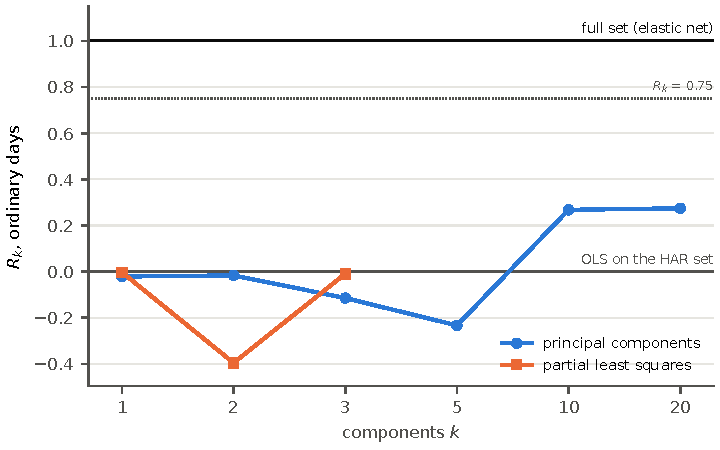
\includegraphics[width=0.75\linewidth]{figures/rehaul_factor_recovery.pdf}
\caption{Share of the full set's ordinary-day gain recovered by $k$ components: $R_k = (L_{\mathrm{HAR}} - L_k)/(L_{\mathrm{HAR}} - L_{\mathrm{full}})$ on the \rhfaNOrdDays{} ordinary days (QLIKE), for OLS on the HAR set plus the first $k$ principal components (blue) or partial least squares components (orange) of the \rhfaNBlock{} non-FOMC value averages. $R_k = 1$: the full set (Table~\ref{tab:rh_oos}'s \rhfaFullOrdModel{}); $R_k = 0$: the OLS on the HAR set. Dotted: $R_k = \rhfaShareThreshold$. Reading: \rhfaReading{} (Table~\ref{tab:rh_factor}).}
\label{fig:rh_factor}
\end{figure}
